\documentclass[11pt]{article}

% Math
\usepackage{amsmath, amssymb, amsfonts, mathtools}

% Page layout
\usepackage[margin=1in]{geometry}

% Optional useful packages
\usepackage{physics}      % \bra, \ket, \dv, \pdv, etc.
\usepackage{bm}           % bold math symbols
\usepackage{bbm}
\usepackage{enumitem}     % better lists
\usepackage{graphicx}     % Required for inserting images
\usepackage{subcaption}   % Required for the subfigure environment
\usepackage{hyperref}     % links
\hypersetup{
    colorlinks=true,       % false: boxed links; true: colored links
    linkcolor=blue,        % color of internal links (sections, pages, etc.)
    citecolor=green,       % color of citation links to bibliography
    % filecolor=magenta,     % color of file links
    urlcolor=blue,         % color of external website links
    % allcolors=blue       % uncomment this if you want ALL links to use one color
}

\title{Weekly Update}
\author{Reza Asakereh}
\date{Last Update: \today}

\begin{document}

\maketitle

\section{Main Findings}
\subsection{DB-Sorter}
\textbf{quick background.} DB-sorter uses the sorting characteristic of DB flow to find ground state or excited states of a hamiltonian $H$ using a diagonal matrix $D$ that has an engineered order in its diagonal elements (usually increasing). \textbf{We can derive Grover's algorithm using DB-Sorter}
\\

\textbf{Findings:}
\begin{itemize}
    \item Grover's algorithm can be improved drastically by replacing its normal reflection method with other diagonal $D$'s. The traditional $I - 2\ket{0}\bra{0}$ Operator needs multiple control phase shift which results in $\mathcal{O}(n^2)$ CNOT's this can be avoided. Also overshoot issue can be managed this way. See \href{https://github.com/rasakereh/double-bracket-algo/blob/master/examples/grover.py}{GitHub} for code and \hyperref[sec:grover]{3.1.1} for figures.
\end{itemize}

\subsection{Fidelity Witness}
\textbf{quick background.} I am working on finding a new fidelity witness. This week effort was through the intermediate step:
\begin{align}
\forall O:  F(P, Q) \ge F(P, O)^2 + F(O, Q)^2 - 1
\label{eq:fidelity-ineq}
\end{align}
It means, for creating a witness, we need to find an $O$ for which we can easily compute any $F(O, Q)$.
\\

\textbf{Findings.}
\begin{itemize}
    \item I assessed Gaussian $O$'s, but with what we already have, they do not seem promising candidates. See \hyperref[sec:gaussian-fidelity]{3.2.1}
    \item Using \textbf{Classical Shadows} we can have a concise classical representation of $P$ and $Q$. They also give us a reasonable approximation for $F(O, P)$ classically. This reduces finding $O$ to a classical optimization. \hyperref[sec:classical-shadow]{3.2.2}
    \item This bound is pretty loose. Intuitively, we need to find an $O$ close enough to both $P$ and $Q$ (e.g $F(P, O) > 0.7$) otherwise the right hand side of the inequality is negative which is trivial.
\end{itemize}



\section{Plan For Next Week(s)}
\subsection{DB-sorter}
\begin{itemize}
    \item finding proper $D$ that guarantees monotone error drop in $\frac{d}{dt}(\bra{k} H(t) \ket{k} - E_k)^2$ for all $k$'s and not just ground state
    \item If $U$ is the unitary transforming $H(0)$ to $H(t)$, finding the fidelity $U\ket{0}$ and the ground state(s) to see if the prepared state constantly converges to a single ground state or is a superposition of degenerate states. Same for the $k$'th excited state
    \item How many steps for Grover's algorithm?
\end{itemize}

\subsection{Fidelity Witness}
\begin{itemize}
    \item explore classical shadows even more and see how far we can go with them
\end{itemize}

\section{Details}
\subsection{DB-sorter}
\subsubsection{Grover's algorithm and DB-sorter}
\label{sec:grover}
In last week's update we see that we can derive Grover's algorithm using DB-sorter. Here I implemented this comparison. This change allow us to change $D$ and $s$ and come up with variations of Grover's algorithm.
Here we compare traditional Grover's algorithm with the case that we replace $I - 2\ket{0}\bra{0}$ projection with a diagonal matrix with ascending elements and $s=1$ with $s=.5$. There are two benefits and one draw-back:
\begin{enumerate}
    \item The depth of the circuit drops significantly. It especially shows up as the number of qubit grows and qubit connections drop as we replace CNOT gates with single-qubit gates.
    \item We easen up on the overshoot problem
    \item The number of steps to convergence is harder to calculate?
\end{enumerate}

In \hyperref[fig:grid_main]{Figure 1} you see how overshoot happens with reflection variation (top row) but not with the monotone $D$ (bottom row)
\begin{figure}[htbp]
    \centering
    % === FIRST ROW ===
    \begin{subfigure}[b]{0.45\textwidth}
        \centering
        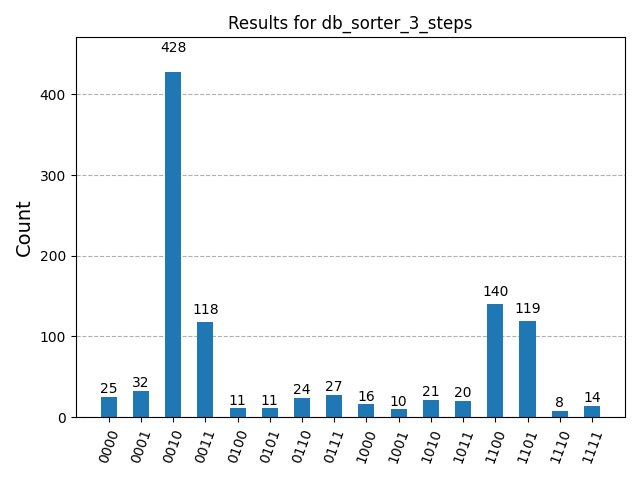
\includegraphics[width=\textwidth]{reflection_3_steps.png}
        \caption{Traditional Grover converged.}
        \label{subfig:reflect-3}
    \end{subfigure}
    \hfill
    \begin{subfigure}[b]{0.45\textwidth}
        \centering
        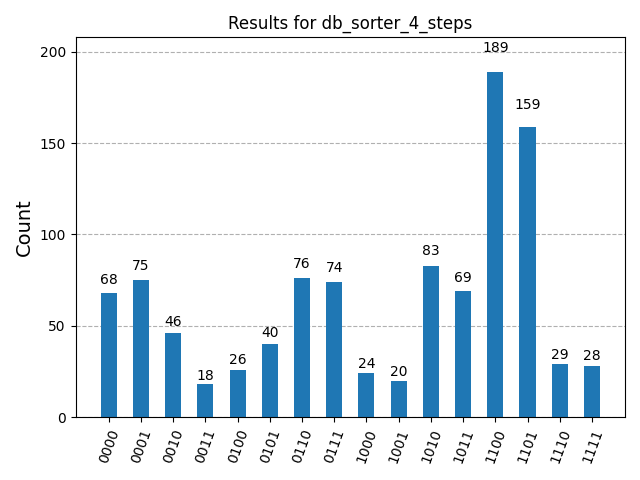
\includegraphics[width=\textwidth]{reflection_4_steps.png}
        \caption{Traditional Grover lost convergence.}
        \label{subfig:reflect-4}
    \end{subfigure}
    
    \vspace{0.5cm} % Adds vertical spacing between the rows
    
    % === SECOND ROW ===
    \begin{subfigure}[b]{0.45\textwidth}
        \centering
        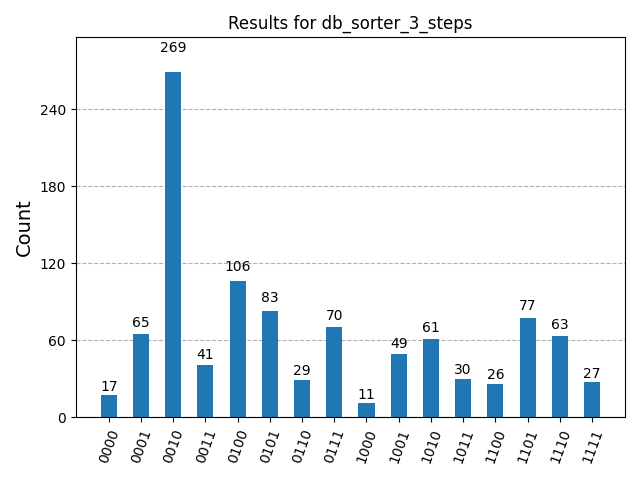
\includegraphics[width=\textwidth]{monotone_3_steps.png}
        \caption{Modified Grover converged.}
        \label{subfig:monotone-3}
    \end{subfigure}
    \hfill
    \begin{subfigure}[b]{0.45\textwidth}
        \centering
        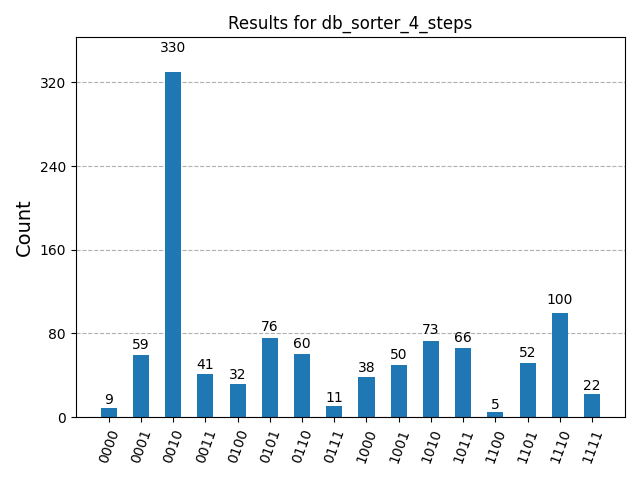
\includegraphics[width=\textwidth]{monotone_4_steps.png}
        \caption{Modified Grover is more resistance to divergence.}
        \label{subfig:monotone-4}
    \end{subfigure}

    % === MAIN CAPTION ===
    \caption{Convergence and divergence in Grover's variations. Marked state: $\ket{0010}$}
    \label{fig:grid_main}
\end{figure}

In \hyperref[fig:grid_main]{Figure 2} you can compare the grover's circuit size in traditional and our variation for the same number of iterations

\begin{figure}[htbp]
    \centering
    % === FIRST ROW ===
    \begin{subfigure}[b]{0.9\textwidth}
        \centering
        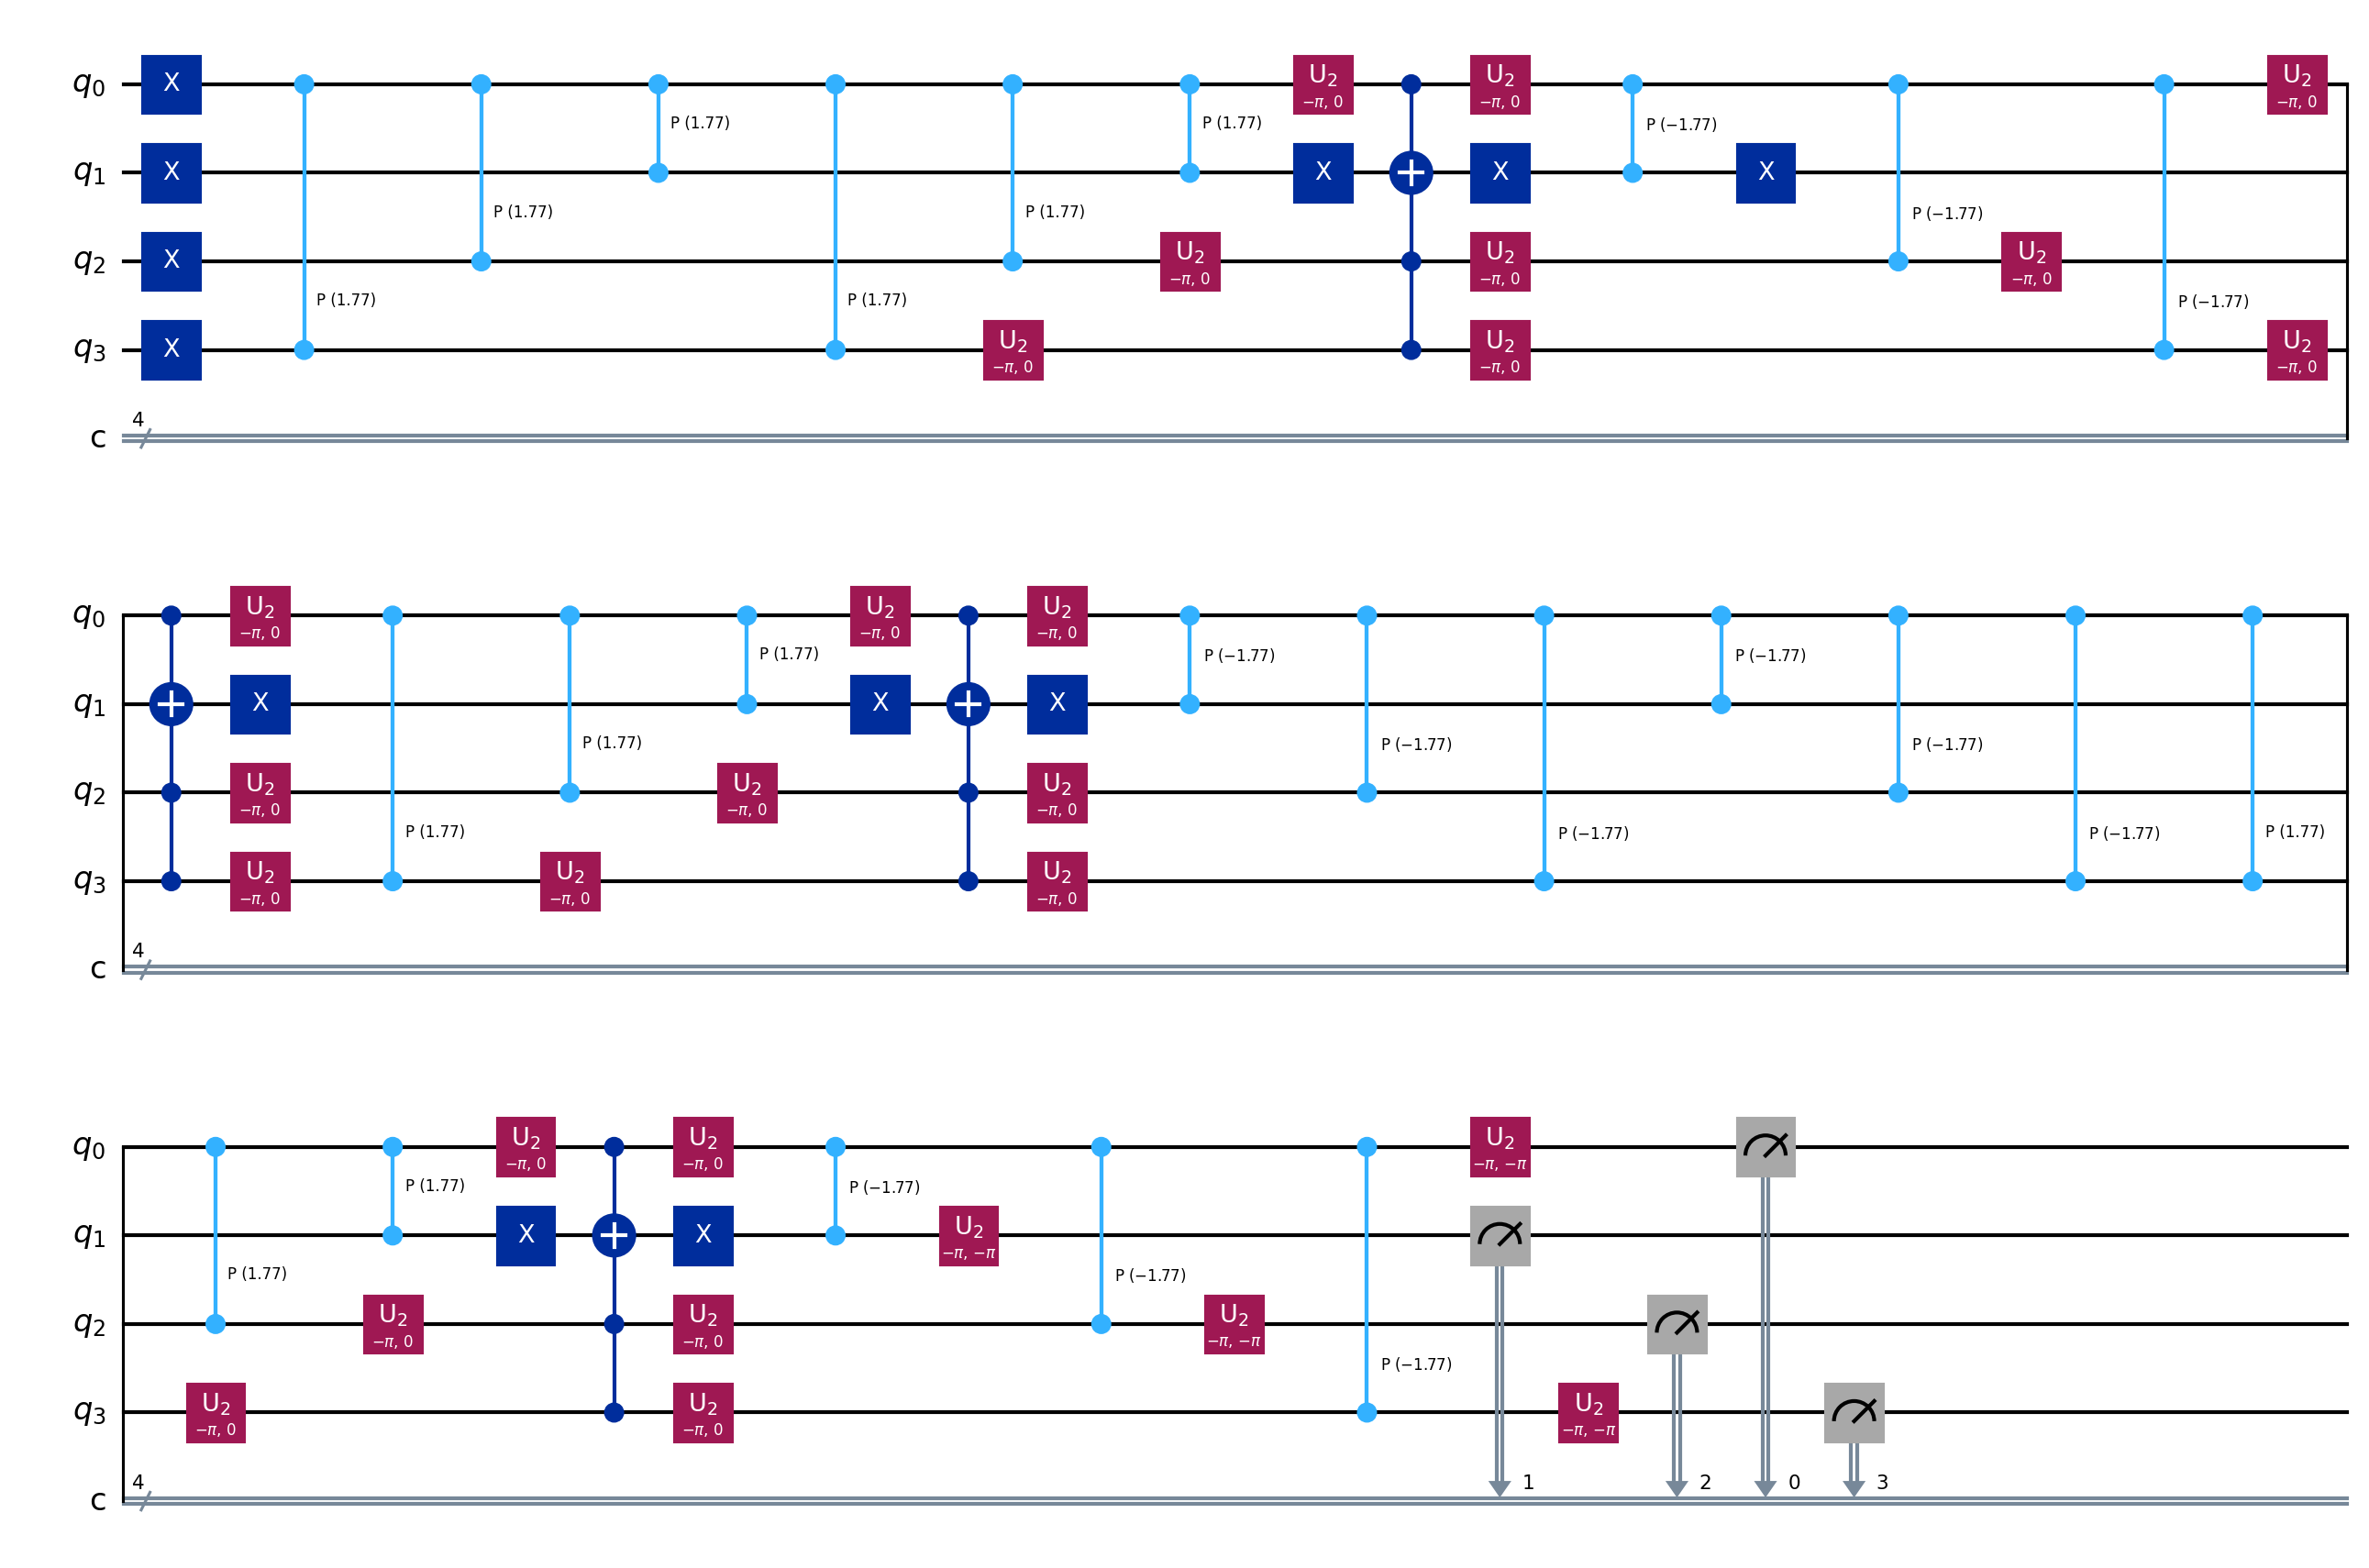
\includegraphics[width=\textwidth]{reflection_transpiled.png}
        \caption{Larger Circuit size due to CNOTs required for $I - 2\ket{0}\bra{0}$.}
        \label{subfig:r-transpile-2}
    \end{subfigure}
    
    \vspace{0.5cm} % Adds vertical spacing between the rows
    
    % === SECOND ROW ===
    \begin{subfigure}[b]{0.9\textwidth}
        \centering
        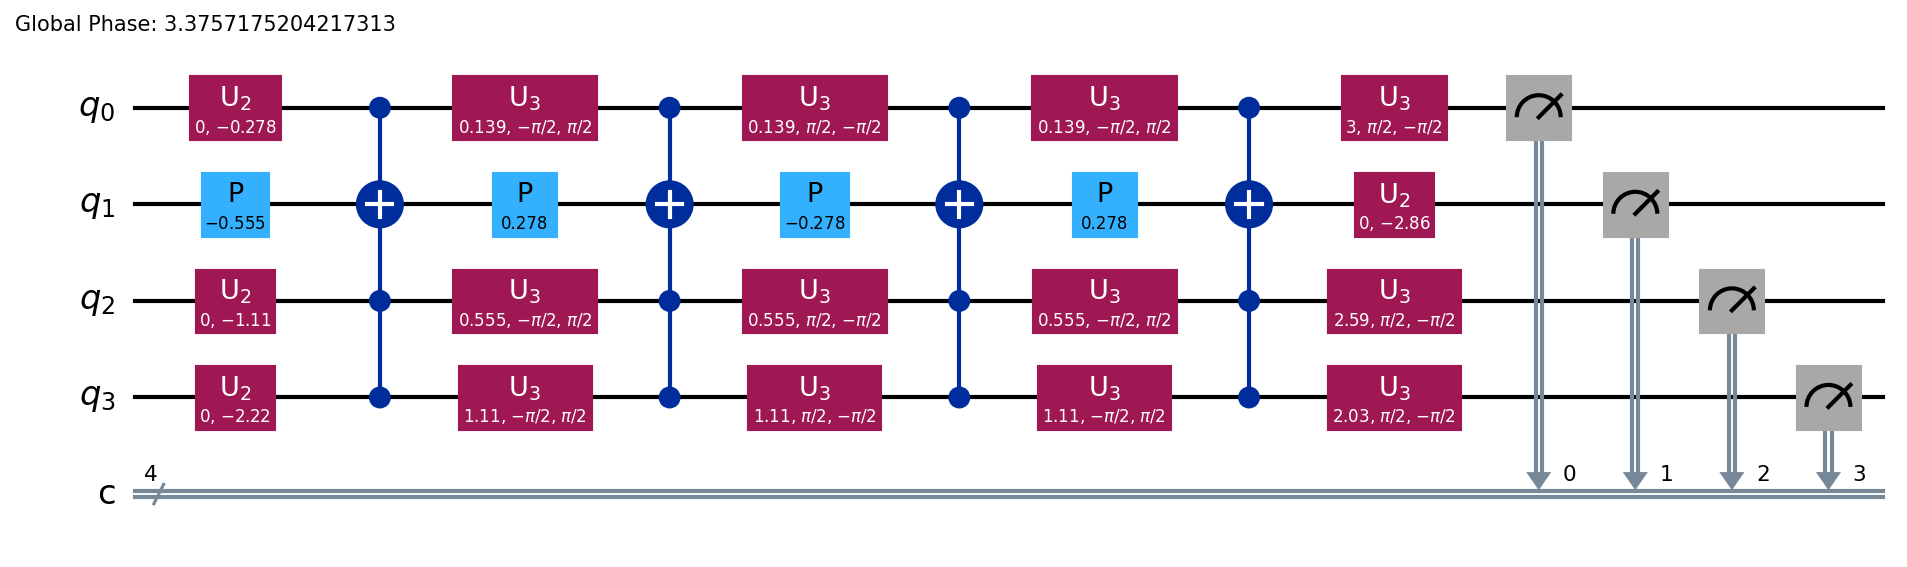
\includegraphics[width=\textwidth]{monotone_transpiled.png}
        \caption{Shallower circuit due to replacing CNOTs with single-qubit gates}
        \label{subfig:m-transpile-2}
    \end{subfigure}

    % === MAIN CAPTION ===
    \caption{We can control Grover's depth by controlling $D$ in DB-Sorter}
    \label{fig:grid_main}
\end{figure}


\subsection{Fidelity Witness}
\subsubsection{Gaussian Fidelity Variational}
\label{sec:gaussian-fidelity}
We already have a Gaussian witness. In \hyperref[eq:fidelity-ineq]{eq-1}, therefore, it is tempting to have a variational optimization in the Gaussian state space. However, it will run into an issue as our witness relies on $\mathcal{W_\omega} = (\mathbf{1} - n_\omega)$. We know that for states with a Hamming distance more than one with $\omega$, the lower bound can be negative, therefore the square would change the direction of the inequality and does not fit our use case.

\subsubsection{Classical Shadow Optimization}
\label{sec:classical-shadow}
\href{https://doi.org/10.48550/arXiv.2002.08953}{Classical shadows} are shown to be useful in capturing major information of state $\rho$ in a set of classical snapshots and use them to estimate $Tr(O\rho)$ for any observable $O$. However the sample size for this relies on how complex $O$ is. Generally, we need exponentially many samples from $\rho$. However for specific classes of observables (e.g separable, unentangled $O$) we can do so polynomially. The advantage of this method is that we do not need to know $O$ in advance; we can store many classical snapshots of $\rho$ and use them for the observables that come to our way. This way, as a witness for $F(P, Q)$, we can capture many snapshots from $P$ and $Q$ and classically optimize the left hand side of the equation $\hat{F}(P, O)^2 + \hat{F}(O, Q)^2 - 1$ where $\hat{F}$ is an estimate of fidelity using classical shadow. The optimization is a classical gradient descend (with normalization in each step to make sure $O$ stays a valid density matrix). The problem here is finding a proper $O$ that is close enough to both $P$ and $Q$ otherwise the sum of squares is less than 1 and only thing we get will be $F(P, Q) > 0$. 
\textbf{Similar work:} The author of classical shadow method have themselves \href{https://doi.org/10.48550/arXiv.2404.07281}{published a paper} for fidelity estimation between any states $P$ (prepared) and $Q$ (target) as long as at least one of them is pure. My method has two advantage and one disadvantage compared to theirs:
\begin{enumerate}
    \item pro: my method can handle both $P$ and $Q$ to be mixed states
    \item pro: their method requires knowledge to all coefficients of the target aka $\bra{k}Q\ket{k}$ which \textit{usually} requires either exponential copies of $Q$ or exponential memory to store these values
    \item con: my method assumes we can produce polynomial copies from the target state while theirs rely only on 1 (i mean they have the coefficients, so...)
\end{enumerate}
The code is attached as a zip file but because for now I am still dealing with finding a better $O$ I still haven't pushed it to the repo as a code structure.



\end{document}
